\setcounter{chapter}{2}

\chapter{微分中值定理与导数的应用}

微分学最初是独立于积分学的,因为其自身已经可以解决许多的应用问题。
本章讨论的极值、最值、单调性和曲率等,都是微分学的独立应用,其中
中值定理和Taylor公式又可以说是整个微分学的“制高点”,集成和融汇
了导数与微分的绝大部分思想与概念,正确地理解和熟练掌握这部分的知识
是对微积分有一个全面深刻认识的基础。

\section{微分中值定理}

中值定理在微分学中是一个非常富于技巧性和魅力的领域,我接下来我们所介绍的
从Rolle定理、Lagrange中值定理、Cauchy中值定理到Taylor公式的演进
路径,真正地将微分学推向了发展和应用的顶峰。

\subsection{Rolle定理}

{\kaishu Fermat引理}:若函数$f(x)$在$x_0$处可导,且在$x_0$的某邻域内,有
$$f(x)\geq f(x_0)\quad (\mbox{或}\quad f(x)\leq f(x_0))$$
则$f'(x_0)=0$。

[证]:设当$x\in U_0(x_0,\delta)$时,总有$f(x)\geq f(x_0)$,则
当$x>x_0$时,总有
$$\df{f(x)-f(x_0)}{x-x_0}\geq 0,$$
而当$x<x_0$时,总有
$$\df{f(x)-f(x_0)}{x-x_0}\leq 0,$$
由极限的保号性,分别令$x\to x_0^+$和$x\to x_0^-$,则有
$$f'(x_0)\geq 0,\quad\mbox{且}\quad f'(x_0)\leq 0,$$
由此即知$f'(x_0)=0$。\hfill$\Box$

\begin{shaded}
	{\bf 关于Fermat和Fermat's Last Theorem}
	
	Pierre de Fermat(1601-1665),法国律师和业余数学家。
	他在数学上的成就不比职业数学家差,他似乎对数论最有兴趣,亦对现代微积分的建立有所贡献。
	\begin{itemize}
	  \setlength{\itemindent}{1cm}
	  \item 微积分:{\it 费马引理}
	  \item 将阿波罗尼奥斯的几何分析中用代数方法来重新建立,开出{\it 解析几何}之路。
	  (费马只使用一轴,只接受正数的答案。后世多以笛卡尔为解析几何的创立者,
	  主因是费马没有发表其作品。)
	  \item 1654年,和Pascal在书信中的讨论,被认为是{\it 概率论}的开端,
	  1656年和概率论的正式创立者Christiaan Huygens(1629-1695)的交流,
	  使后者增加了对概率论的兴趣
	\end{itemize}
	
	Fermat{\it 小定理}:假设$a\in\mathbb{Z}$,$p$为素数,则$a^p-a$可以整除$p$,
	或者写为
	$$a^p\equiv a(\mathrm{mod}p),$$
	特别低,若$a$不是$p$的倍数,则上式可写为$a^{p-1}\equiv 1(\mathrm{mod} p)$
	
	Fermat小定理是RSA公钥加密体制的理论基础,如果没有公钥加密体制,信息技术将
	不可能呈现今天的面貌。下面的是Fermat最重要的一个猜想,也是最后被证明的一个猜想。
	
	Fermat{\it 大定理}(也称Fermat最后定理):对于大于$2$的正整数$n$,以下方程
	无正整数解
	$$x^n+y^n=z^n.$$
	这个定理造成了数学史上最大的悬案:1637年,费马在阅读丢番图《算术》拉丁文译本时,
	曾在第11卷第8命题旁写道:
	{\it 将一个立方数分成两个立方数之和,或一个四次幂分成两个四次幂之和,
	或者一般地将一个高于二次的幂分成两个同次幂之和,这是不可能的。
	关于此,我确信已发现了一种美妙的证法,可惜这里空白的地方太小,写不下。}
	
	一直被称为“Fermat猜想”,直到英国数学家Andrew John Wiles及其学生Richard
	Taylor于1995年将他们的证明出版后,才称为“Fermat大定理”。
	经过数学家们三个多世纪的努力,猜想才变成了定理。在冲击这个数论世纪难题的过程中,
	无论是不完全的还是最后完整的证明,都给数学界带来很大的影响;很多的数学结果、
	甚至数学分支在这个过程中诞生了,包括代数几何中的{\it 椭圆曲线}和{\it 模形式},
	以及{\it	Galois理论}和{\it Hecke代数}等。这也令人怀疑
	当初费马是否真的找到了正确证明。
	
	\begin{itemize}
	  \setlength{\itemindent}{1cm}
	  \item 1770年,Euler证明 $n=3$时定理成立
	  \item 1823年,Legendre证明$n=5$时定理成立
      \item 1832年,Dirichlet试图证明$n=7$失败,但证明$n=14$时定理成立
	  \item 1839年,Gabriel Lamé证明$n=7$时定理成立
	  \item 1850年,Ernst Eduard Kummer证明$2<n<100$时除$37$、$59$、$67$三数外定理成立
	  \item 1955年,Harry Vandiver以电脑计算证明了对所有不超过$2521$的素数定理成立
	  \item 1976年,Samuel Wagstaff以电脑计算证明对所有不超过$125000$的素数定理成立
	  \item 1985年,电脑计算证明了对所有小于$4$百万的素数定理成立
	  \item 1987年,格朗维尔以电脑计算证明了$2<n<10^{{1800000}}$时定理成立
	  \item 1995年,Wiles证明$n>2$时定理成立。
	\end{itemize}
	
	Wiles证明Fermat大定理的过程亦甚具戏剧性。他用了七年时间,在不为人知的情况下,
	得出了证明的大部分;然后于1993年6月在一个学术会议上宣布了他的证明,并瞬即
	成为世界头条。但在审批证明的过程中,专家发现了一个极严重的错误。Wiles和他的学生Taylor
	然后用了近一年时间尝试补救,终在1994年9月以一个之前Wiles抛弃过的方法得到成功。
	
	为什么Fermat大定理在数学史上的地位如此重要?有三个主要的原因:一是问题基本,长时间
	(350年)悬而未决,吸引了众多数学大师对其加以研究;二是研究问题的过程中产生了新的思想和方法,
	带动了数学很多领域的发展;三是涉及Taniyama-Shimura theorem({\it 谷山—志村猜想}),
	是现代数学大热门Langlands program({\it 朗兰兹纲领})的重要组成部分。1967年提出的
	Langlands program指出三个相对独立发展起来的数学分支:数论、代数几何和群表示论,
	实际上是密切相关的,而连接这些数学分支的纽带是一些特别的函数,被称为L-函数。
	L-函数可以说是Langlands program的中心研究对象。数学界著名的七个
	{\it “千禧年大奖问题”}(Millennium Prize Problems)中有两个就是关于L-函数的,
	它们分别是{\it Riemann假设}和{\it BSD猜想}。
	
	延伸阅读:
	\begin{enumerate}[1.]
	  \setlength{\itemindent}{1cm}
	  \item 知乎:为什么费马大定理在数学史上的地位如此重要?
	  \item 知乎:为什么费马大定理表述起来这么简单,证明却这么复杂?
	  \item https://en.wikipedia.org/wiki/Fermat's\_Last\_Theorem
	  \item https://zh.wikipedia.org/wiki/费马大定理
	  \item https://en.wikipedia.org/wiki/Andrew\_Wiles
	  \item https://en.wikipedia.org/wiki/Pierre\_de\_Fermat
	  \item 推翻费马大定理!https://st.im/wGX
	  \item 又一千禧年大奖难题被攻破,下一个向P/NP进发吧!https://st.im/wGL
	\end{enumerate}
\end{shaded}

{\kaishu Rolle定理:}若函数$f(x)$满足:
\begin{enumerate}[(1)]
  \setlength{\itemindent}{1cm}
  \item 在区间$[a,b]$上连续;
  \item 在区间$(a,b)$内可导;
  \item $f(a)=f(b)$。
\end{enumerate}
则:存在$\xi\in(a,b)$,使得$f\,'(\xi)=0$。

[证]:$f(x)$在$[a,b]$上连续,故必存在最大和最小值,由于$f(a)=f(b)$,
故除非$f(x)\equiv f(a)$(此时定理显然成立),最大和最小值点不可能
同时为$a$和$b$,故必存在某个$\xi\in(a,b)$为$f(x)$的一个最值点。
因为$f(x)$在$(a,b)$内可导,故由Fermat引理,必有$f'(\xi)=0$,即证。\hfill$\Box$

{\bf 注:}{\b 三个条件缺一不可!!}\ps{为什么?每种情况给出相应的反例!}

\begin{center}
	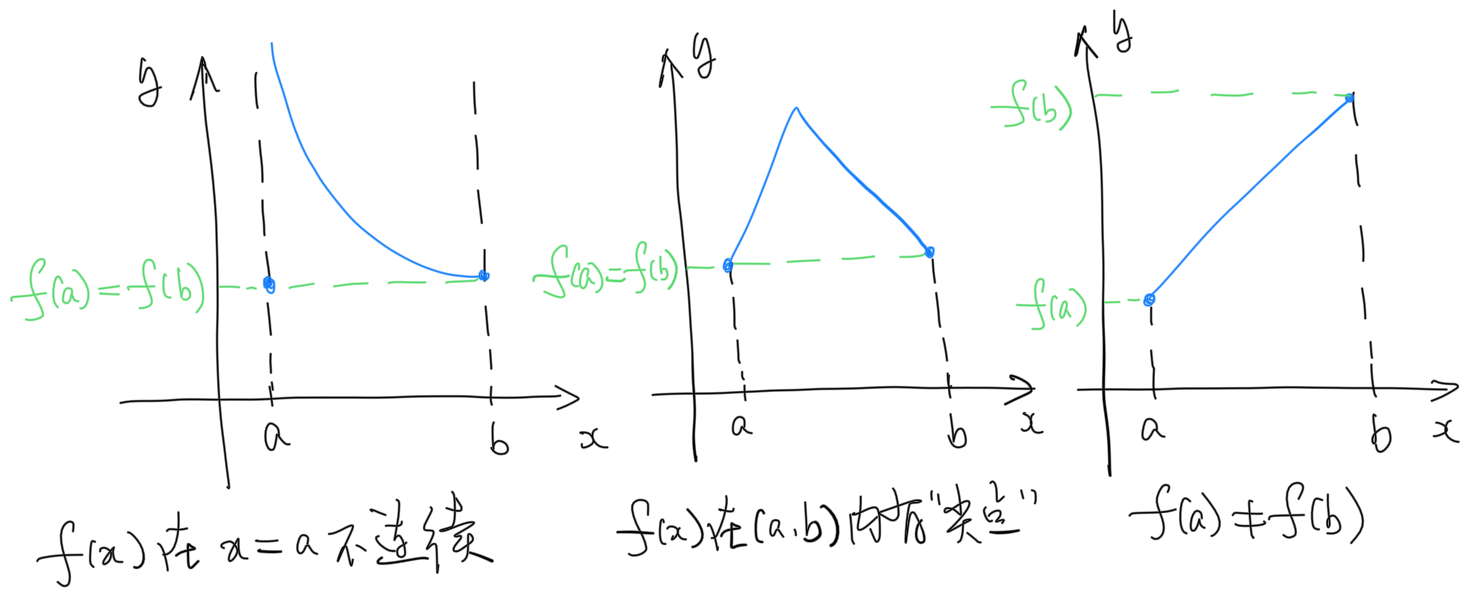
\includegraphics[width=0.9\textwidth]{./images/ch3/antiRolle.jpg}
\end{center}

{\bf 例:}证明:对函数$f(x)=(x-1)(x-2)(x-3)$,至少存在一点
$\xi\in(1,3)$,使得$f\,''(\xi)=0$。

[证]:$f(x)$是任意阶可导的,且在$[1,2],[2,3]$上均满足Rolle定理条件,
故必存在$\xi_1\in(0,1),\xi_2\in(2,3)$,使得
$$f'(\xi_1)=f'(\xi_2)=0.$$
进一步地,容易验证$f'(x)$在$[\xi_1,\xi_2]$上满足Rolle定理条件,
故必存在$\xi\in(\xi_1,\xi_2)$,使得$f''(\xi)=0$。
\hfill$\Box$

参照这个例题的证明思路,可以很容易地得到如下的推论:

{\kaishu Rolle定理的高阶推广}:
设$f(x)$在$[x_0,x_n]$上有$n-1$阶连续导函数,在$(x_0,x_n)$内
$n$阶可导,且
$$f(x_0)=f(x_1)=\ldots=f(x_n),\quad(x_0<x_1<\ldots<x_n),$$
则存在$\xi\in(x_0,x_n)$,使得$f^{(n)}(\xi)=0$。

利用Rolle定理证明可以证明一些有趣的结论,也可以构造出很多看似花样百出
的{\it 存在性问题}:

[提示]:利用极限的保号性,说明在$a,b$附近各有一点,两点函数值反号,然后利用
介值定理和Rolle定理。

{\bf 例:}设$\df{a_0}{n+1}+\df{a_1}{n}+\ldots+a_n=0$,证明:方程
$$a_0x^n+a_1x^{n-1}+\ldots+a_n=0$$
在区间$(0,1)$内至少有一个根。

[提示]:令
$$F(x)=\df{a_0}{n+1}x^{n+1}+\df{a_1}{n}x^n+\ldots+a_nx$$

{\bf 例:}设$f(x)\in C[a,b]$,在$(a,b)$内可导,且$f(a)=f(b)=0$,证明:存在
$\xi\in(a,b)$,使得:
$$f'(\xi)+f(\xi)=0.$$

[提示]:$F(x)=f(x)e^x$

{\bf 注:}{\b 辅助函数的构造可以从不定积分中获得一些启发
\begin{itemize}
  \setlength{\itemindent}{1cm}
  \item $f(\xi)+\lambda f'(\xi)=0$:令$F(x)=e^{\lambda x}f(x)$
  \item $f'(\xi)+f(\xi)g'(\xi)=0$: 令$F(x)=e^{\lambda g(x)}f(x)$
  \item $nf(\xi)+xf'(\xi)=0$: 令$F(x)=x^nf(x)$ 
  \item $f'(\xi)g(\xi)+f(\xi)g'(\xi)=0$:令$F(x)=f(x)g(x)$
  \item $f'(x)g(x)-f(x)g'(x)=0$: 令$F(x)=\df{f(x)}{g(x)}$
\end{itemize}
}

{\bf 例}({\kaishu Darboux定理})设$f(x)$在$[a,b]$上可导,
且$f\,'_+(a)f\,'_-(b)<0$,则存在$\xi\in(a,b)$,使得$f\,'(\xi)=0$。

\begin{center}
	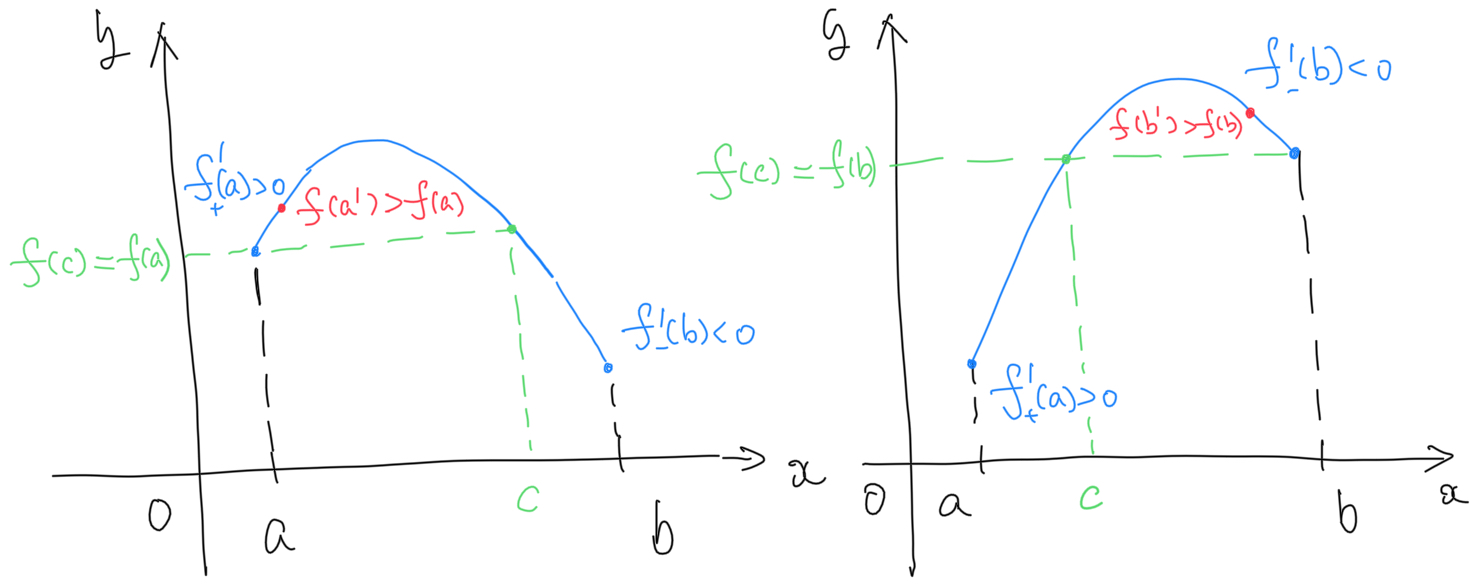
\includegraphics[width=0.9\textwidth]{./images/ch3/Darboux.jpg}
	
	\it Darboux定理的证明思路
\end{center}

[证]:不妨设$f'_+(a)>0$,且$f(a)>f(b)$(如左图)。

由$f'_+(a)>0$,也即$\limx{a^+}\df{f(x)-f(a)}{x-a}>0$,
由极限的保号性,必存在某个$a'>a$,使得$\df{f(a')-f(a)}{a'-a}>0$,
进而$f(a')>f(a)$。

显然$f(x)$在$[a',b]$上连续,$f(a)\in(f(b),f(a'))$,故由介值定理,
必存在$c\in(a',b)$,使得$f(c)=f(a)$。
注意到$f(x)$在$[c,b]$上满足Rolle定理条件,故必存在$\xi\in(c,b)\subset(a,b)$,
使得$f'(\xi)=0$。\hfill$\Box$

Darboux定理说明导函数具有{\it 介值性},即可以证明:介于区间端点处的导数值之间的所有
导数值,都可以在区间内部的某点上取到\ps{请自行尝试证明}。
介值性和连续性的关系一度是微积分理论中的难题,人们曾经猜想介值性和连续性是等价的,
直到发现不连续的导函数(例如:$f(x)=x^2\sin\frac1x$的导函数在$x=0$不连续),
并且通过Darboux定理验证了导函数的介值性,才发现这个猜想是错误的。

{\bf 思考题:}设$f(x)$在$[a,b]$上满足Rolle定理条件,
且$f\,'_+(a)f\,'_-(b)>0$,则$f\,'(x)=0$在$(a,b)$内至少有两个根。

\begin{center}
	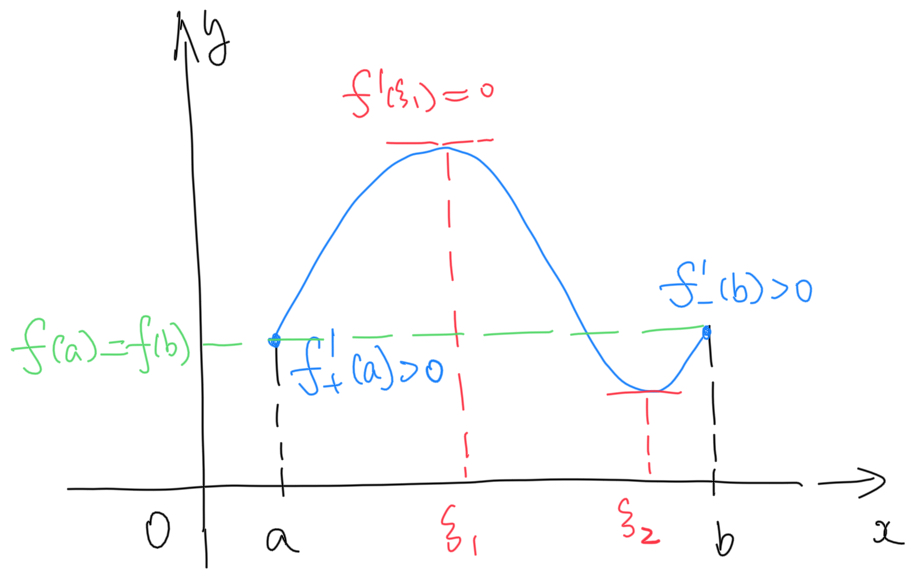
\includegraphics[width=0.6\textwidth]{./images/ch3/Darboux2.jpg}
	
	\it 示意图
\end{center}
[提示]:先利用Rolle定理证明存在$\xi_1$,再根据$f(\xi_1)$与$f(a)$的大小关系,
采用与证明Darboux定理类似的方法证明$\xi_2$的存在。

\subsection{Lagrange中值定理}

{\kaishu Lagrange中值定理}:若函数$f(x)$满足:\ps{这个定理据说实际上是由Cauchy证明的}
\begin{enumerate}[(1)]
  \setlength{\itemindent}{1cm}
  \item 在区间$[a,b]$上连续 
  \item 在区间$(a,b)$内可导 
\end{enumerate}
则:{\b 存在$\xi\in(a,b)$,使得 
$$f\,'(\xi)=\df{f(b)-f(a)}{b-a}.$$}

[提示]:结论即为\ps{\b 从结论出发构造辅助函数是证明中值问题的常用思路}
$$f'(\xi)(b-a)-[f(b)-f(a)]=0,$$
考虑
$$F'(x)=f'(x)(b-a)-[f(b)-f(a)],$$
则
$$F(x)=f(x)(b-a)-[f(b)-f(a)]x+C,$$
不妨令$C=0$,可以验证$F(b)=F(a)=bf(a)-af(b)$,再利用Rolle定理即可。

关于该证明的构造思路,有着非常生动形象的几何解释,具体请参见教材。从图示上看,
新构造的$F(x)$相当于是将原来的$f(x)$两端“拉平”(按比例平移)后得到的,
这种变换的一个重要特点是变换前后两个函数的连续性和可导性完全一致。

然而,从我们的分析过程来看,求解此类题目,完全不需要任何几何的直观,
可以直接从结论出发,通过求导的逆向过程(也就是{\it 不定积分})来构造出
所需的辅助函数。

Lagrange中值定理的结论有时也写作:{\b 存在$(\theta\in(0,1))$,使得}
$${\b f(x+\Delta x)=f(x)+f'(x+\theta\Delta x)\Delta x.}$$

{\bf 例:}证明:
\begin{enumerate}[(1)]
  \setlength{\itemindent}{1cm}
  \item 导数恒为零的函数取值恒为常数。
  \item 导数恒大于零的函数严格单调递增。
\end{enumerate}

{\bf 例:}证明方程$x^5+x-1=0$只有唯一实根。

{\bf 例:}证明:$\df{\ln x-\ln x_1}{x-x_1}<\df 1{x_1},\quad (0<x_1<x)$

{\bf 例:}证明不等式:$\df{x}{1+x}<\ln(1+x)<x,\;x>0$

% {\bf 注:}在证明Eular常数
% $$\gamma=\limn\left(1+\df12+\ldots+\df1n-\ln n\right)$$
% 时,用到了这个不等式。

{\bf 例:}设$f(x)\in C[a,b]$,且$f(x)$在$(a,b)$内二阶可导,
连接函数曲线两端点的直线在$(a,b)$内至少与曲线存在一个交点,
则存在$\xi\in(a,b)$,使得$f\,''(\xi)=0$。

{\bf 思考:}{\b 若函数曲线的端点连线与函数曲线存在多个交点,能够得到什么结论?}

{\bf 例:}设$f(x)$在$[a,b]$上二阶可导,$f(a)=f(b)=0$,证明:对任意
$c\in(a,b)$,存在$\xi\in(a,b)$,使得
$$f(c)=\df{f\,''(\xi)}{2}(c-a)(c-b)$$

[提示]:设
$$F''(x)=f''(x)-\df{2f(c)}{(c-a)(c-b)},$$
则可得
$$F(x)=f(x)-\df{f(c)}{(c-a)(c-b)}x^2+C_1x+C_2,$$
其中$C_1,C_2$为常数。不妨令$C_1=C_2=0$,以下可以验证:
$$\df{F(c)-F(a)}{c-a}=\df{F(b)-F(c)}{b-c}
=-\df{f(c)}{(c-a)(c-b)}(a+b),$$
由Lagrange中值定理,存在$\xi_1\in(a,c),\xi_2\in(c,b)$,使得
$$F'(\xi_1)=F'(\xi_2)=-\df{f(c)}{(c-a)(c-b)}(a+b),$$
进而再由Rolle定理,存在$\xi\in(\xi_1,\xi_2)$,使得$F''(\xi)=0$,即证。

[注]:直接令辅助函数
$$F(x)=f(x)-\df{(x-a)(x-b)}{(c-a)(c-b)}f(c)$$
亦可,这个辅助函数的右半部分事实上是过$(a,0),(b,0),(c,f(c))$
三点的{\kaishu Lagrange插值多项式}!

\begin{shaded}
{\bf 过$n$个点$(x_i,f(x_i))(i=1,2,\ldots,n)$的Lagrange插值多项式}
$$L_n(x)=\sum\limits_{i=1}^n\prod_{j=1,j\ne i}^{n}
\df{x-x_j}{x_i-x_j}f(x_i)$$

插值可以理解成利用一条曲线在给定的点之间“穿插”,而插值多项式就是用于穿插
(连接)所有给定点的一个多项式函数。在工程应用中,对离散的观测数据进行建模,
得到反映变化(运动)规律的函数曲线,从而对未来的变化(运动)趋势进行预测,
是很常见的问题。

{\bf 例:}过点$(0,0),(1,2),(2,-1),(3,-2)$的Lagrange插值多项式为
$$L(x)=\df{x^3}6-8x^2+\df{41}6x$$

\begin{center}
	\resizebox{!}{5cm}{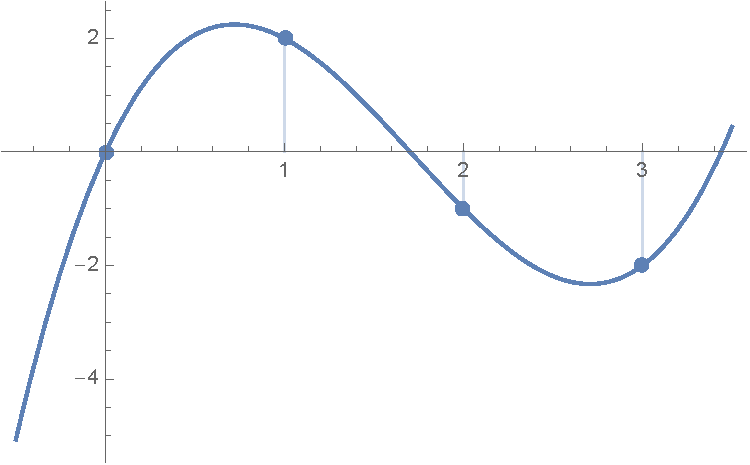
\includegraphics{./images/ch5/L4x.pdf}}
\end{center}
%% code of Mathematica 
% f[x_] := 7/6*x^3 - 6 x^2 + 41/6*x;
% CCurve = Plot[f[x], {x, -0.5, 3.5}];
% DCurve = ListPlot[Table[{n, f[n]}, {n, 0, 3}], Filling -> Axis];
% Show[CCurve, DCurve]

\end{shaded}

\subsection{Cauchy中值定理}

{\kaishu Cauchy中值定理}:若函数$f(x),\varphi(x)$满足: 
\begin{enumerate}[(1)]
  \setlength{\itemindent}{1cm}
  \item 在$[a,b]$上连续 
  \item 在$(a,b)$内可导,且$\varphi'(x)\ne 0$ 
\end{enumerate}
则:存在$\xi\in(a,b)$, 使得
$$\df{f(b)-f(a)}{\varphi(b)-\varphi(a)}=\df{f'(\xi)}{\varphi'(\xi)}$$

[提示]:结论即为
$$[f(b)-f(a)]\varphi'(\xi)-[\varphi(b)-\varphi(a)]f'(\xi)=0,$$
因此考虑
$$F'(x)=[f(b)-f(a)]\varphi'(x)-[\varphi(b)-\varphi(a)]f'(x),$$
从而
$$F(x)=[f(b)-f(a)]\varphi(x)-[\varphi(b)-\varphi(a)]f(x)+C.$$
不妨令$C=0$,可以验证$F(b)=F(a)$,利用Rolle定理即可。

这个证明思路延续了我们此前证明很多中值问题所使用的方法,与教材上的方法存在
比较明显的差异,但从解题的角度来看,更具普遍的可操作性。

{\bf 注:}Cauchy中值定理可视为{\it 参数化}的Lagrange中值定理,即:
由$\varphi'(x)\ne 0$可知,$\varphi(x)$为单调(可逆)函数,从而设
$A=\varphi(a),B=\varphi(b)$,故由Lagrange中值定理,存在$\xi\in(a,b)$,
也即$C=\varphi(\xi)$介于$A,B$之间,使得
$$\df{f(b)-f(a)}{\varphi(b)-\varphi(a)}
=\df{f(\varphi^{-1}(B))-f(\varphi^{-1}(A))}{B-A}
=[f(\varphi^{-1}(x))]'_{x=\xi}=\df{f'(\xi)}{\varphi'(\xi)}.$$

{\bf 综合练习}:
{\bf 例:}设$0<a<b$,$f(x)$在$[a,b]$上连续,在$(a,b)$内可导,证明:
\begin{enumerate}[(1)]
  \setlength{\itemindent}{1cm}
  \item 存在$\xi\in(a,b)$,使得:
	$$f(b)-f(a)=\ln\df ba\cdot \xi f\,'(\xi)$$
  \item 存在$\eta\in(a,b)$,使得:
    $$2\eta[f(b)-f(a)]=(b^2-a^2)f\,'(\eta)$$
  \item 存在$x_1,x_2,x_3\in(a,b)$,使得
	$$f\,'(x_1)=(b+a)\df{f\,'(x_2)}{2x_2}=(a^2+ab+b^2)
	\df{f\,'(x_3)}{3x_3^2}$$ 
  \item 若$f\,'(x)\ne 0$,则存在$\xi,\eta\in(a,b)$,使得
	$$\df{f'(\xi)}{f'(\eta)}=\df{e^b-e^a}{b-a}e^{-\eta}$$
  \item 存在$c\in(a,b)$,使得
	$$\df{1}{a-b}\left|\begin{array}{cc}
	a & b\\ f(a) & f(b)
	\end{array}\right|=f(c)-cf'(c).$$
\end{enumerate}

通过对结论适当变形整理,以上结论都可以使用Rolle定理证明。

\section{L'Hospital法则}

\section{Taylor公式}

\section{函数的单调性与凹凸性}

\subsection{单调性的判定}

\subsection{凹凸性与拐点}

\section{函数的极值与最值}

\subsection{极值}

\subsection{最值问题}

\section{分析绘图}

\section{曲率}

\subsection{弧微分}

\subsection{曲率的定义}

\subsection{曲率的应用}

极限是微积分理论体系中最基本也最重要的概念之一,后面我们将要讨论的导数(微分)和
积分的概念都是建立在极限概念之上的,更具体地说,导数和定积分都是特定类型的极限。

在上一章学习了数列极限的基础上,本章我们将进一步讨论更具一般性的函数的极限,二者
的定义和性质,从很多方面来看都是相似的,只是由于函数极限的类型更为丰富,相对而言
有关结论也更为多样,有些性质是数列极限所不具备的。

\section{函数极限的概念与性质}

函数极限是我们后续定义导数、积分的概念的基础,因此可以说函数极限的理论也是整个
微积分学的基础。



\section{函数极限的判敛}

\subsection{四则运算}

{\bf 定理3.2.1:}若函数极限存在,则极限运算可以和四则运算交换次序。

{\bf 注:}把握两点
\begin{itemize}
  \setlength{\itemindent}{1cm}
  \item 有限次四则运算
  \item 可以推广到初等函数
\end{itemize}







\subsection{夹逼定理}


\section{无穷大、无穷小和函数的渐近线}

在求解(函数)极限的问题中,分子分母同时趋于零
\ps{所谓不定是相对诸如有界量乘以无穷小(趋于零)、有界量除以无穷大一类容易确定的形式而言的}
(例如:$\limx{0}\df{\cos
x-\cos2x}{x^2}$),或者一个趋于零的函数和一个趋于无穷的函数的乘积(例如:$\limx{+\infty}x^2e^-x$)
的极限通常是较难求解的,这类问题我们称之为“$\df00$”和“$0\cdot\infty$” 型的{\it 不定式(极限)}!


{\bf 思考:}除了“$\df00$”和“$0\cdot\infty$”型的不定式,还可能有其他形式的不定式吗?

{\bf 答:}有,型如:“$\df{\infty}{\infty}$”、“$1^{\infty}$”、“$0^0$”,例如:
$\limx{+\infty}\df{\ln x}{x}$,$\limx{\infty}\left(1+\df1{x}\right)^{\sin
x}$,$\limx{0}x^{2x}$

\subsection{无穷大和无穷小}

{\bf 定义3.3.1:}$f(x)$是$x\to\Delta$时的无穷小$\Leftrightarrow\limx{\Delta}f(x)=0$

{\bf 注:}$\Delta$可任意代表$\infty,\;+\infty,\;-\infty,\;x_0,\;x_0^+,\;x_0^-$之一

{\bf 定理3.3.1-3.3.2}(无穷小的性质)
\begin{enumerate}[(1)]
  \setlength{\itemindent}{1cm}
  \item $\limx{\Delta}f(x)=A\in\mathbb{R}\Leftrightarrow
  f(x)-A$是$x\to\Delta$时的无穷小
  \item $x\to\Delta$时的有界函数与无穷小之积仍为$x\to\Delta$时的无穷小
  \item $x\to\Delta$时的有限个无穷小之和(积)仍为$x\to\Delta$时的无穷小
\end{enumerate}

{\bf 定义3.3.2:}$f(x)$是$x\to\Delta$时的无穷大$\Leftrightarrow\limx{\Delta}\df 1{f(x)}=0$,
可记为:
$$\limx{\Delta}f(x)=\pm\infty$$

{\bf 注:}{\b 无穷大有正负之分!!}

{\bf 【渐近线】}\ps{具体内容请阅读教材自学!}

$x\to x_0$时的无穷大意味着存在{\it 铅直渐近线};$x\to\pm\infty$时的无穷大
{\it 可能}意味着存在{\it 斜渐近线},例如:若$y=f(x)$当$x\to+\infty$时的
存在斜渐近线$y=kx+b$,则
$$k=\limx{+\infty}\df{f(x)}x,\quad b=\limx{+\infty}[f(x)-kx].$$
注意,{\b $x\to\pm\infty$时的斜渐近线可能是不同的!}例如:$y=x\arctan x$趋于
$x\to\pm\infty$时的斜渐近线分别为$y=\pm\df{\pi}2x$.

% {\bf P129-例4:}证明:$x+\sin x$是$x\to\infty$时的无穷大

{\bf 定理3.3.3:}在$x\to\Delta$的同一过程中:
\begin{enumerate}[(1)]
  \setlength{\itemindent}{1cm}
  \item 有界函数与无穷大之和仍为无穷大
  \item 有限个无穷大之乘积仍为无穷大({\it 但可能反号})
\end{enumerate}

{\bf 例:}证明:$f(x)=a_0x^n+a_1x^{n-1}+\ldots+a_n(n\in\mathbb{N})$
是$x\to\infty$时的无穷大,其中:$a_0,a_1,\ldots,a_n\in\mathbb{R},a_0\ne 0$

\begin{shaded}
	{\bf 无穷大之间的比较!}
	
	当$x\to+\infty$时,存在如下的大小关系:设$a>0$,
	$$\ln x<<x^a<<e^x<<\Gamma(x)<<x^x$$
	其中$\Gamma-$函数定义为$\Gamma(x)=\dint_0^{+\infty}t^{x-1}e^{-t}\d t$,
	满足$\Gamma(n)=(n-1)!,\;(n\in\mathbb{Z}_+)$
\end{shaded}

\subsection{无穷小的比较}



\subsection{斜渐近线}

若$y=f(x)$当$x\to+\infty$时以$y=kx+b$为斜渐进线,则有
$$k=\limx{+\infty}\df{f(x)}{x}=k,\quad b=\limx{+\infty}[f(x)-kx]$$

{\bf 例:}求曲线$y^2-x^2=2x$的渐近线。

{\bf 教材3.3.4节-例10:}求函数$f(x)=\df{2x^2-3}{x+1}$的渐近线。

\begin{center}
	\resizebox{!}{5cm}{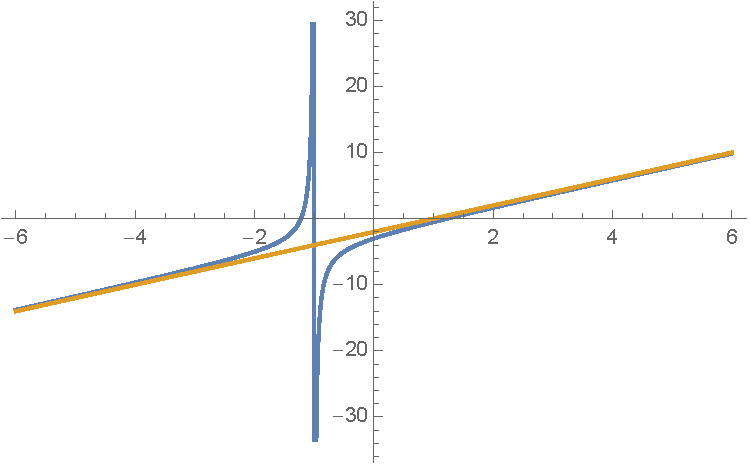
\includegraphics{./images/ch3/asyx.pdf}}
\end{center}

\section{函数的连续性}



\subsection{基本性质}

{\bf 定理3.4.1-3.4.4:}


\subsection{连续函数在有界闭区间上的性质}

\subsubsection{【最值定理】}


\subsubsection{【介值定理】}



% \section*{补充例题}
% \addcontentsline{toc}{section}{补充例题}
% 
% {\bf 例}:证明函数$f(x)=\left\{\begin{array}{ll}
% x,\;&x\in\mathbb{Q}\\ 0,\;&\mathrm{else}
% \end{array}\right.$
% 仅在$x=0$连续
% 
% {\bf 证:}显然$f(0)=0$。注意到
% $$0<|f(x)|\leq |x|,$$
% 而$\lim\limits_{x\to 0}|x|=0$,故由夹逼定理
% $$\lim\limits_{x\to 0}f(x)=0=f(0),$$
% 也即$f(x)$在$x=0$连续。
% 
% \bigskip
% 
% 设$x_0\ne 0$,下证$\lim\limits_{x\to x_0}f(x)$不存在,进而可知
% $f(x)$在$x_0$处不连续。事实上,若设$\lim\limits_{x\to x_0}f(x)$存在,
% 则
% $$\lim\limits_{x\to x_0}D(x)=\frac{\lim\limits_{x\to x_0}f(x)}
% {\lim\limits_{x\to x_0}x}$$
% 也存在,从而与$D(x)$在任意点处极限不存在矛盾。
% 
% 综上,$f(x)$仅在$x=0$连续。
% 
% \newpage
% 
% \newpage



\newpage

\section*{课后作业}
\addcontentsline{toc}{section}{课后作业}

{\bf 【必作题】}

\begin{itemize}
  \item 习题3.1:4(1,3),7,15
  \item 习题3.2:2,3,4,5
  \item 习题3.3:2,4,5,7(2,6),8,9,10(3,4)
  \item 习题3.4:5(1-3),9,15,17
\end{itemize}

\bigskip

\hrule

\bigskip
\bigskip

{\bf 【思考题】}
\begin{itemize}
  \item 习题3.1:10,11,12
  \item 习题3.2:6,7
  \item 证明:$$\limn\left\{\lim\limits_{m\to\infty}\left[\cos^{2m}(n!\pi
	x)\right]\right\}=D(x)$$
	其中$D(x)$为Dirichlet函数
%   \item 自学3.3.3节:渐近线 
  \item 习题3.3:1,6,12,13
  \item  计算极限
  \item 习题3.4:1,3,13,14,16,19
  \item 设$a_1<a_2<\ldots<a_n$,证明以下方程有$n-1$个实根
	$$\df 1{x-a_1}+\df 1{x-a_2}+\ldots+\df 1{x-a_n}=0.$$
\end{itemize}

\newpage

\section*{补充例题}
\addcontentsline{toc}{section}{补充例题}



{\bf 例:}设$f(x)$在$x_0$的某邻域内有定义,且$x_0$为其间断点,则下列函数
必以$x_0$为间断点的是(B)

\quad
(A)\;$f(x)\sin x$\hspace{2cm}
(B)\;$f(x)+\sin x$\hspace{2cm}
(C)\;$f^2(x)$\hspace{2cm}
(D)\;$|f(x)|$ 

{\bf 例:}设$x\to 0$时,$e^{\tan x}-e^x$与$x^n$为同阶无穷小,则$n$=(C)
\ps{Taylor展开}

\quad
(A)\;$1$\hspace{2cm}
(B)\;$2$\hspace{2cm}
(C)\;$3$\hspace{2cm}
(D)\;$4$ 

{\bf 例:}设$x\to 0$时,$x-\sin ax$与$x^2\ln(1-bx)$为同阶无穷小,则(A)
\ps{Taylor展开}

\quad
(A)\;$a=1,b=-\df16$\hspace{1em}
(B)\;$a=1,b=\df16$\hspace{1em}
(C)\;$a=-1,b=-\df16$\hspace{1em}
(D)\;$a=-1,b=\df16$

{\bf 例:}若$f(x)=\df{\sqrt[3]{x}}{\lambda-e^{-kx}}$在$(-\infty,+\infty)$
上连续,且$\limx{+\infty}f(x)=0$,则(D)

\quad
(A)\;$\lambda<0,k<0$\hspace{1cm}
(B)\;$\lambda<0,k>0$\hspace{1cm}
(C)\;$\lambda\geq0,k<0$\hspace{1cm}
(D)\;$\lambda\leq0,k>0$

% \begin{tabbing}
% 	\hspace{3cm}\=\hspace{3cm}\=\hspace{3cm}\=\kill
% 	\quad\quad\quad
% 	(A)\;$\lambda<0,k<0$\>  
% 	\quad\quad\quad
% 	(B)\;$\lambda<0,k>0$\>
% 	\quad\quad\quad  
% 	(C)\;$\lambda\geq0,k<0$\>
% 	\quad\quad\quad 
% 	(D)\;$\lambda\leq0,k>0$
% \end{tabbing} 

{\bf 例:}设$f(x)$在$(a,b)$内均有定义且单调有界,则$f(x)$在$(a,b)$内的间断点类型只能是(C)
\begin{tabbing}
	\hspace{8cm}\=\kill
	\quad\quad\quad
	(A)\;可去间断点 \> 
	(B)\;第二类间断点 \\ 
	\quad\quad\quad
	(C)\;跳跃间断点\>
	(D)\;不能确定
\end{tabbing}



{\bf 例:}



{\bf 例:}设$x\in(0,1]$时,$f(x)=x^{\sin x}$,且对任意$x$
$$f(x)+k=2f(x+1),$$
求常数$k$的值,使得极限$\limx0f(x)$存在。

[提示]:易知$\limx{0^+}f(x)=1$,有$x\in(-1,0]$时,
$$f(x)=2(x+1)^{\sin(x+1)}-k,$$
故$\limx{0^-}f(x)=2-k$,从而可得$k=1$.

{\bf 例:}设$f(x)$在$[a,b]$上连续,$\{x_n\}$为$[a,b]$上任一数列,求
$\limn\sqrt[n]{\df1n\sum\limits_{k=1}^ne^{f(x_k)}}$

[提示]:$e^{f(x)}$在$[a,b]$上连续且非负,故可设$m,M$分别为其在$[a,b]$上的最大和最小值,
从而由夹逼定理
$$\sqrt[n]m\leq\sqrt[n]{\df1n\sum\limits_{k=1}^ne^{f(x_k)}}\leq\sqrt[n]M,$$
由此易知原式$=1$。
